\subsection{命令模式(Command)}

\subsubsection{命令模式简介}

命令模式是一种设计模式,它把请求封装成对象,允许你把请求参数化,并且提供了一种为不同的请求设置不同的撤销和恢复操作的能力。

例如,假设你正在开发一个文本编辑器。在文本编辑器中,用户可以执行操作,例如撤销上一次操作和恢复上一次撤销的操作。为了实现这个功能,你可以使用命令模式,将每个操作封装成一个命令对象,然后把这些对象存储在一个历史记录中。这样,用户就可以撤销和恢复之前的操作了。

另一个例子是电视遥控器。你可以把遥控器的每个按钮看作一个命令,当用户按下按钮时,遥控器就会执行相应的操作。这样,用户可以通过按钮来控制电视,而不用关心具体的操作细节。

总之,命令模式提供了一种将请求封装成对象的方式,使得你可以将请求参数化,并且提供了撤销和恢复操作的能力。

命令模式的优点是:
\begin{enumerate}
    \item 命令模式将请求封装成对象,使得你可以对请求进行参数化。
    \item 命令模式提供了一种撤销和恢复操作的能力。
    \item 命令模式使得你可以轻松地实现日志和撤销功能。
    \item 命令模式可以把复杂的操作拆分成多个步骤,每个步骤都是一个命令,这样可以方便地实现复杂操作的撤销和恢复。
\end{enumerate}

命令模式的缺点是:
\begin{enumerate}
    \item 命令模式会增加系统的复杂度,因为它把请求封装成对象,增加了系统中对象的数量。
    \item 命令模式需要额外的存储空间来保存命令历史记录,以便支持撤销和恢复操作。
    \item 如果命令执行失败,撤销和恢复操作可能会带来一定的困难。
\end{enumerate}
上面这些缺点并不会导致命令模式无法使用,但是在使用命令模式时需要注意这些缺点,并采取适当的措施来应对这些缺点。例如,你可以通过合理地设计系统来减少对象的数量,或者采用更高效的数据结构来存储命令历史记录,以减少存储空间的消耗。

\subsubsection{命令模式在项目中的应用}

\begin{figure}[h]
    \centering
    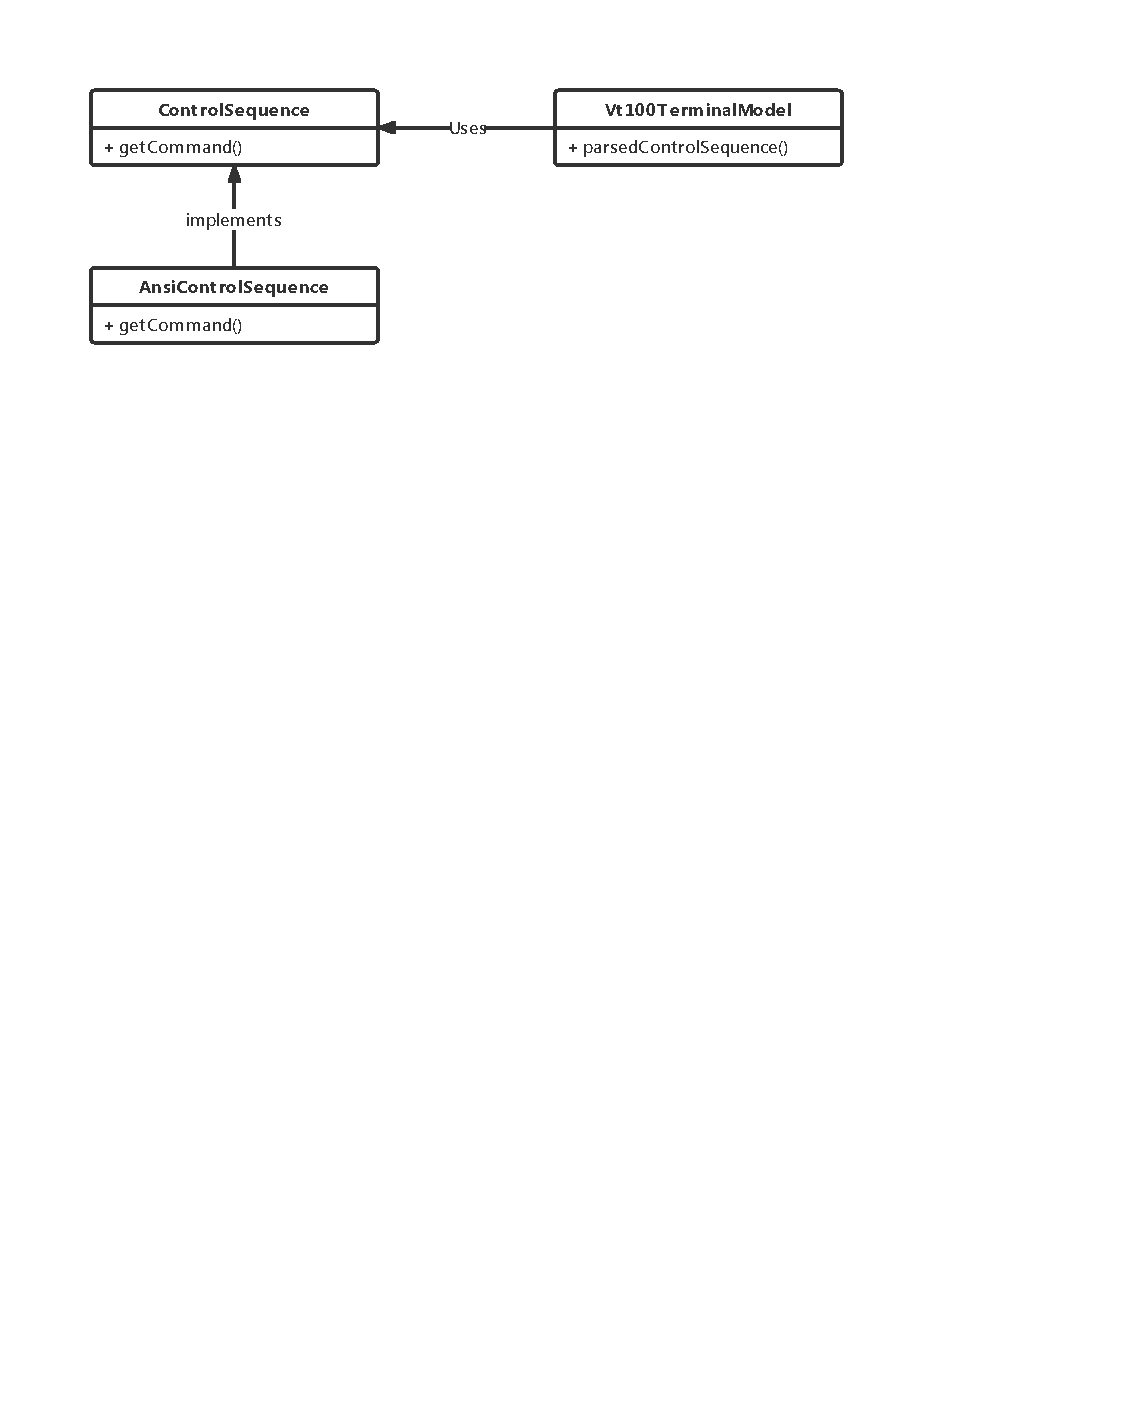
\includegraphics[width=0.9\textwidth]{figures/Command.pdf}
    \caption{命令模式在 Slow6502 中的类图}
\end{figure}

在我们的项目中,我们使用命令模式来抽象终端外设的 Ansi Control Sequence。这样就可以方便地对 ANSI 控制序列进行参数化,从而避免使用硬编码的 ANSI 控制序列。

